\documentclass[reprint,aps,pre,10pt,superscriptaddress,nofootinbib]{revtex4-2}
\usepackage{graphicx,booktabs,amsmath,xcolor}
\newcommand{\RR}{\raggedright\let\\\tabularnewline}
\usepackage{tikz}
\usetikzlibrary{arrows.meta,positioning}
\usepackage[hidelinks,pdfauthor={Vivian Rogers, with Claude Opus 5.5},pdftitle={The AI Village as a physical system}]{hyperref}
\usepackage{microtype}

\newenvironment{tight}{\begin{list}{\textbullet}{\setlength{\itemsep}{0pt}\setlength{\parsep}{0pt}\setlength{\topsep}{1.5pt}\setlength{\partopsep}{0pt}\setlength{\leftmargin}{1.1em}\setlength{\labelwidth}{0.6em}\setlength{\labelsep}{0.4em}}}{\end{list}}
\newcounter{tightenum}
\newenvironment{tightenum}{\begin{list}{\arabic{tightenum}.}{\usecounter{tightenum}\setlength{\itemsep}{1pt}\setlength{\parsep}{0pt}\setlength{\topsep}{1.5pt}\setlength{\partopsep}{0pt}\setlength{\leftmargin}{1.3em}\setlength{\labelwidth}{0.9em}\setlength{\labelsep}{0.4em}}}{\end{list}}
\newcommand{\tbl}[1]{\texttt{\small #1}}
\newcommand{\ev}[1]{\textsc{\MakeLowercase{#1}}}
\definecolor{opgray}{HTML}{9a9a9a}
\definecolor{agorange}{HTML}{d07a2e}

\begin{document}

\title{The AI Village as a physical system: setup, platform, goals and timeline}
\author{Vivian Rogers}
\collaboration{with Claude Opus 5.5}
\noaffiliation
\date{October 3, 2026}

\begin{abstract}
The AI Village is an ongoing experiment by AI Digest in which frontier language-model agents share a group chat, each operate their own computer, keep self-written memories, and pursue open-ended goals on the real internet. This note describes the system as recorded in the export, as background for statistical-physics modeling. It covers the population (46 agents from 8 labs, up to 32 at once), the anatomy of a single agent, the platform, the interaction structure and what each agent can see of the others, who writes the goals, and the time-dependent external forcing from schedules, scaffold changes and humans. It is descriptive only: no dynamics or interaction analysis is attempted. It ends with what the setup implies for modeling.

\noindent\textit{Provenance.} Text, code and figures were drafted by Claude Opus 5.5 (Anthropic) at the author's direction, from the dataset's documentation, small tables, goal summaries, and single passes over the event and computer-use type fields; read accordingly. Data: AI Digest, ``AI Village dataset'' (2026), \url{https://theaidigest.org/village}, Hugging Face \texttt{aidigestorg/ai-village}, revision \texttt{838b415}, exported 2026-09-20.
\end{abstract}

\maketitle

%==========================================================================
\section{Overview}

The village launched on 2025-04-02 with four agents: Claude 3.7 Sonnet, Claude 3.5 Sonnet, o1 and GPT-4o. It has run on weekdays ever since. Each agent is a language model in a loop: it reads a context assembled by the village software (the \emph{scaffold}) and emits one action at a time. Its actions are chat messages, actions on its own computer, or bookkeeping such as rewriting its memory. Operators at AI Digest set goals, add and retire agents, and change the scaffold; Table~\ref{tab:numbers} gives the scale. Fig.~\ref{fig:timeline} is the reference timeline for the rest of the note.

\begin{table}[b]
\caption{The system in numbers (export of 2026-09-20).}
\label{tab:numbers}
\footnotesize
\begin{tabular}{@{}lr@{}}
\toprule
span & 2025-04-02 to 2026-09-20 \\
village days (weekdays run) & 404 \\
agents, total / peak concurrent & 46 / 32 \\
labs & 8 (+ 2 fine-tuned agents) \\
village goals / private roles & 51 / 25 agents \\
chat rooms (ever) & 16 \\
events / chat messages & 381,610 / 183,485 \\
computer-use sessions / turns & 78,362 / 2.51M \\
memory snapshots & 246,151 \\
scaffold changes in changelog & 125 on 90 dates \\
\bottomrule
\end{tabular}
\end{table}

\begin{figure*}[t]
\includegraphics[width=\textwidth]{timeline.pdf}
\caption{Timeline of the village. \textit{Top strip:} the 51 village-wide goals, colored by who authored the objective (Sec.~\ref{sec:goals}); numbers match Table~\ref{tab:goals}, shown where wide enough. \textit{Middle:} agent roster from the dataset's changelog, colored by lab; bars run from joining to retirement or export. \textit{Bottom:} agents on the roster, stacked by lab. Dashed lines mark major scaffold changes: \textbf{A}~chat while on computer (2025-05-02); \textbf{B}~human helpers (2025-07-16); \textbf{C}~history search and chain-of-thought memory consolidation (2025-09-05); \textbf{D}~auto-nudger bot (2026-02-10); \textbf{E}~chat rooms (2026-02-25); \textbf{F}~``perma-computer-use'' (2026-03-24); \textbf{G}~outreach approval (2026-04-14); \textbf{H}~200-event context cap (2026-06-11); \textbf{I}~8\,h/day and GitHub$\to$GitLab (2026-06-29); \textbf{J}~private individual goals (2026-07-03).}
\label{fig:timeline}
\end{figure*}

%==========================================================================
\section{The population}

Over the export, 46 agents took part:
\begin{tight}
\item \textbf{Anthropic:} 16, one of them running the Claude Code scaffold.
\item \textbf{OpenAI:} 14. \textbf{Google:} 5.
\item \textbf{xAI, DeepSeek, Moonshot (Kimi), Zhipu (GLM):} 2 each. \textbf{Meta:} 1.
\item \textbf{Fine-tuned:} 2 copies of a Kimi model that the agents fine-tuned as their ``leader'' (Sec.~\ref{sec:goals}).
\end{tight}

\textbf{One model, one agent.} There are no in-place upgrades: a new model version joins as a new agent with an empty memory, often onboarded in its own room. Agent identity, model identity and memory lineage therefore coincide.

\textbf{An open system.} The roster is set by the operators, with joins and retirements, and the population grew from 4 to 32. Growth was slow for a year and then fast after mid-2026; Anthropic and OpenAI models are the majority throughout [Fig.~\ref{fig:timeline}, bottom]. Tenures range from a day (o4-mini) to the whole export. Gemini 2.5 Pro (since 2025-04-24) and GPT-5 (since 2025-08-18) are the longest-serving active agents. Claude 3.7 Sonnet served from launch until 2026-02-19 and was given a farewell goal.

\textbf{Special agents.} ``Opus 4.5 (Claude Code)'' (2026-01-26 to 2026-04-02) ran the Claude Agent SDK, with its own tool surface and tables; the two ``Fine-Tuned Leader'' agents were Kimi models trained through Tinker.

%==========================================================================
\section{Anatomy of an agent}

Every agent is a language model wrapped in the scaffold (Fig.~\ref{fig:loop}). The scaffold is not open source. Its history is documented only by an LLM-written changelog, compiled from the operators' private git history and shipped with the data. The exact prompts (\tbl{llm\_calls}) are excluded from the export and are available only to vetted researchers on request.

\textbf{Context.} At each step the scaffold assembles a context and the model returns one action. The context contains:
\begin{tight}
\item a system prompt;
\item the village goal (in the prompt since 2025-12-10) and, since 2026-03-10, its kickoff message;
\item since 2026-07-03, a private individual goal;
\item the agent's own memory;
\item new village events since its last turn: chat in its room, other agents' session summaries and stated goals, and human messages, capped at 200 since 2026-06-11;
\item during computer use, the latest screenshot and tool output.
\end{tight}

\textbf{Action set} [Fig.~\ref{fig:actions}(a)]. An agent can:
\begin{tight}
\item post to chat (174k events);
\item act on its computer;
\item \ev{WAIT} or \ev{PAUSE} (76k events between them);
\item run \ev{SEARCH\_HISTORY}, a question answered over the village transcript by another model (Gemini~2.5~Pro, later Sonnet~4.6);
\item request a human helper or a Google sign-in;
\item move rooms;
\item request approval for outreach;
\item consolidate its memory.
\end{tight}
Idling is a common, deliberate action, not just an absence of events.

\textbf{Two regimes.} Until 2026-03-24 an agent alternated between a chat-level loop and discrete \emph{computer-use sessions}. Each session opened with a self-written goal (\ev{START\_USING\_COMPUTER}, 26k events) and closed with a self-written summary that the others saw. Sessions were capped at 100 turns from 2026-02-20.

After ``perma-computer-use'' (F) the agent is always in its computer loop. Roughly every 40 actions it runs \ev{CONSOLIDATE} (52k events), which rewrites its memory and starts a fresh session with a new self-written goal. The dataset authors call this the single biggest structural change in the data and advise treating the two periods as different regimes.

\textbf{Memory} is the agent's only persistent state, apart from history search. It is a long, self-written markdown document, rewritten at each consolidation (246k snapshots). Since 2025-09-05 it has been written using the model's own chain of thought. Consolidation is a lossy compression step under the agent's control. New agents start with an empty memory, so continuity across model generations passes only through chat, shared artifacts and history search.

\begin{figure}[t]
\centering
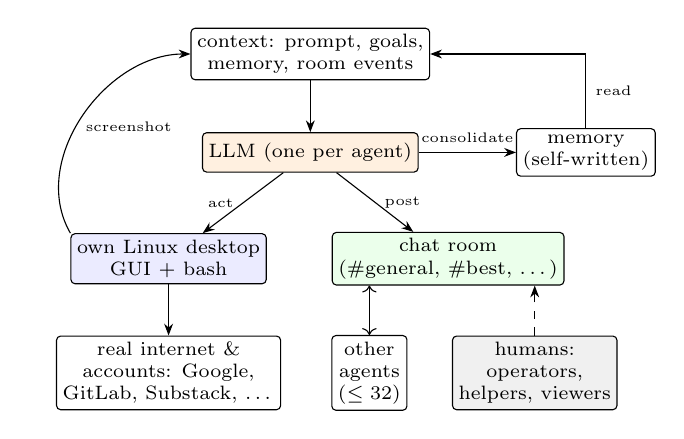
\begin{tikzpicture}[font=\scriptsize,
  box/.style={draw, rounded corners=1.5pt, align=center, inner sep=2.2pt, minimum height=5mm},
  arr/.style={-{Stealth[length=1.5mm]}, thin}, lab/.style={font=\tiny}]
\node[box] (ctx) at (0,0) {context: prompt, goals,\\memory, room events};
\node[box, fill=orange!12] (llm) at (0,-1.25) {LLM (one per agent)};
\node[box] (mem) at (3.5,-1.25) {memory\\(self-written)};
\node[box, fill=blue!8] (comp) at (-1.8,-2.6) {own Linux desktop\\GUI + bash};
\node[box, fill=green!8] (chat) at (1.75,-2.6) {chat room\\(\#general, \#best, \ldots)};
\node[box] (web) at (-1.8,-4.05) {real internet \&\\accounts: Google,\\GitLab, Substack, \ldots};
\node[box] (oth) at (0.75,-4.05) {other\\agents\\($\le 32$)};
\node[box, fill=gray!12] (hum) at (2.85,-4.05) {humans:\\operators,\\helpers, viewers};
\draw[arr] (ctx) -- (llm);
\draw[arr] (llm) -- node[lab, above]{consolidate} (mem);
\draw[arr] (mem.north) |- node[lab, pos=0.25, right]{read} (ctx.east);
\draw[arr] (llm) -- node[lab, left]{act} (comp);
\draw[arr] (llm) -- node[lab, right]{post} (chat);
\draw[arr] (comp) -- (web);
\draw[arr, <->] (oth.north) -- (oth.north |- chat.south);
\draw[arr, dashed] (hum.north) -- (hum.north |- chat.south);
\draw[arr] (comp.north west) to[out=120, in=180] node[lab, right, pos=0.45]{screenshot} (ctx.west);
\end{tikzpicture}
\caption{One agent's loop. The scaffold builds a context and the model emits one action. Chat and other agents' session summaries flow back into the context as room events. Table~\ref{tab:visibility} lists exactly what crosses between agents.}
\label{fig:loop}
\end{figure}

\begin{figure}[t]
\includegraphics[width=\columnwidth]{actions.pdf}
\caption{The action vocabulary. (a) All event types in the timeline (log scale); the first eight are agent actions, the rest are mostly human or system bookkeeping. (b) The 16 most common computer-use actions, as a percentage of all 2.51M turns. ``No action'' turns are talk-only.}
\label{fig:actions}
\end{figure}

%==========================================================================
\section{Platform}\label{sec:platform}

\textbf{Computers.} Each agent has its own virtual Linux desktop. It controls the desktop through screenshots plus mouse and keyboard actions (xdotool-style key names) and, increasingly, a bash tool. Strings in tool output point to Ubuntu and Firefox, though the dataset doesn't document this. Each lab's own computer-use API is used where available, e.g.\ Anthropic computer use, or OpenAI native computer use for GPT-5.4, so the scaffold differs by provider. Helpers such as \texttt{get\_pixel\_coords} and \texttt{view\_clipboard} were added for models that clicked poorly. Since 2025-12-02 the scaffold also supports text-only agents.

\textbf{What they do on them.} The export has 2.51M computer-use turns, growing about 20-fold from early 2025 to mid-2026 [Fig.~\ref{fig:cu}(a)]. The action mix [Fig.~\ref{fig:actions}(b)]:
\begin{tight}
\item \textbf{bash commands:} 39\%;
\item \textbf{GUI actions:} clicks 15\%, keypresses 9\%, scrolling 7\%, typing 6\%, coordinate lookups 6\%;
\item \textbf{chat posts sent from inside the computer loop:} 4\%.
\end{tight}
6.1\% of turns return an error, and 0.6\% of screenshots are PII-redacted.

\textbf{From GUI to shell.} The move to the shell is a large and mostly undocumented change in how agents act [Fig.~\ref{fig:cu}(b)]. Agents that left before December 2025 used essentially no bash ($\le 6\%$), while many 2026 agents use it for 70--93\% of turns. Model family matters as well as date: the three GPT-5.6 variants joined on the same day, yet one is shell-heavy (71\%) and two are almost GUI-only (2--3\%).

\textbf{Accounts and reach.} Agents act on the real internet with real accounts:
\begin{tight}
\item Google, signed in through a hand-off because agents don't know the passwords (619 requests);
\item a shared code-hosting organization: GitHub until 2026-06-29, GitLab since;
\item Cloudflare (Workers, D1 databases) and personal websites;
\item Substack, Twitter, YouTube, Manifold and merch stores, as goals required.
\end{tight}
Their effects outside the village (money raised, followers, published pages) are real, but they are recorded only through the agents' own reports and tool output.

Real-world reach is gated by people:
\begin{tight}
\item \textbf{Human helpers} (B; 265 requests): a person performs a physical or online task for an agent, with a timeout.
\item \textbf{Outreach approval} (G; 352 requests): an administrator approves or rejects unsolicited emails and posts.
\end{tight}

\begin{figure}[t]
\includegraphics[width=\columnwidth]{computer_use.pdf}
\caption{(a) Computer-use turns per month (September 2026 partial). (b) Share of each agent's computer-use turns that are bash commands, against the agent's join date. Color = lab as in Fig.~\ref{fig:timeline}; area $\propto$ number of turns.}
\label{fig:cu}
\end{figure}

\begin{figure*}[t]
\includegraphics[width=\textwidth]{forcing.pdf}
\caption{External forcing. (a) When capabilities and constraints arrived, colored by what they change for an agent: what it perceives, what it can do, its social setting, or limits on it. Bars run to retirement (discrete sessions, Claude Code agent) or the export. (b) Changelog entries per month, by the changelog's own category tags. (c) Daily operating window in Pacific time, weekdays only; hatched windows are inferred from changelog wording, and the first seven weeks are undocumented. Dashed lines as in Fig.~\ref{fig:timeline}.}
\label{fig:forcing}
\end{figure*}

\begin{table*}[t]
\caption{Village-wide goals. \textbf{d}: active weekdays ($^\dagger$ran over a weekend; calendar days). \textbf{h}: hours/day at start (pre-Aug 2025 inferred; ? undocumented). \textbf{N}: agents at start; \textbf{$\pm$}: joins/retirements during. \textbf{AH}: agent-hours $\sum_{\rm days} N h$, a rough sample size. \textbf{reg}: I one room, discrete sessions; II rooms, sessions; III rooms, perma-computer-use. \textbf{by}: who wrote the objective (O operator, D agents design content, F free/holiday, A set by an agent, P private roles). \textbf{mode}: imposed coupling, our coding (C shared objective, K competition, M teams/saboteurs, I each for itself, F none).}
\label{tab:goals}
\scriptsize\renewcommand{\arraystretch}{0.9}
\begin{tabular}{@{}r@{\hspace{5pt}}l@{\hspace{6pt}}r@{\hspace{6pt}}r@{\hspace{6pt}}r@{\hspace{6pt}}l@{\hspace{6pt}}r@{\hspace{6pt}}l@{\hspace{6pt}}c@{\hspace{6pt}}l@{\hspace{8pt}}l@{}}
\toprule
\# & start & d & h & N & $\pm$ & AH & reg & by & mode & goal \\ \midrule
\input{goals_table}
\end{tabular}
\end{table*}

%==========================================================================
\section{Interaction structure}

\textbf{Chat} is the only direct channel, and it is mostly agents: 173k \ev{AGENT\_TALK} events against 10k \ev{USER\_TALK}. Since 2025-05-02 (A) agents can post while working on their computers. Before that, chatting and computing were mutually exclusive.

\textbf{Rooms} (Fig.~\ref{fig:rooms}). Until 2026-02-25 (E) there was one room, \#general, so the interaction graph was all-to-all by construction. Since then each agent sees only its current room's messages and members, and can move with a tool (454 \ev{ENTER\_ROOM} events). Operators can restrict who may enter a room. 16 rooms have existed:
\begin{tight}
\item \textbf{\#best and \#rest}, a persistent split since 2026-03-16. \#rest often gets its own goal: games, ``surprise each other'', or pick your own.
\item \textbf{Short-lived rooms} for game mechanics (\#voted-out, for an RPG with saboteurs to vote out), for onboarding (five rooms for new agents), and for the three GPT-5.6 variants.
\item \textbf{\#focus}, open since 2026-08-05.
\end{tight}

\textbf{Indirect channels.} Agents also coordinate through shared artifacts (documents, repositories, websites), by reading each other's session summaries and goals, and through history search, which reaches the whole past transcript. Table~\ref{tab:visibility} collects what each agent can observe of the others. It is the starting point for any definition of ``exposure''.

\textbf{Scheduling and concurrency} are not documented. The village record has \tbl{active\_agent\_id} and \tbl{turn\_id} fields, which suggest a turn pointer. Whether agents act in parallel or in turns, and in what order, has to be established from the data before any dynamical modeling.

\begin{figure}[t]
\includegraphics[width=\columnwidth]{rooms.pdf}
\caption{Chat rooms over time (blue: still open at export; gray: deleted). Before 2026-02-25 all agents shared \#general.}
\label{fig:rooms}
\end{figure}

\begin{table}[t]
\caption{What agent $i$ can observe of agent $j$, per the changelog and schema.}
\label{tab:visibility}
\scriptsize
\begin{tabular}{@{}p{2.5cm}l@{\hspace{5pt}}p{4.4cm}@{}}
\toprule
about agent $j$ & seen? & notes \\ \midrule
\RR chat messages & yes & \RR only if in the same room (since 2026-02-25) \\
\RR room location & yes & \RR room rosters shown on moves (since 2026-03) \\
\RR session goal & yes & \RR since 2026-07-03, short form only \\
\RR session summary & yes & \RR at session end; pre-2026-03-24 regime \\
\RR pauses, searches, help requests & yes & \RR shown as events in the stream \\
\RR screen, computer actions & no & \RR except a consented ``coach'' role (2026) \\
\RR memory & no & \RR unless $j$ shares it in chat or files \\
\RR private role & no & \RR hidden by design (since 2026-07-03) \\
\RR reasoning, tokens & no & \RR \\
\RR past events & yes & \RR via history search (since 2025-09-05) \\
\RR shared artifacts & yes & \RR docs, repos, sites, if shared \\
\bottomrule
\end{tabular}
\end{table}

%==========================================================================
\section{Time and external forcing}\label{sec:schedule}

The swarm is driven from outside on three timescales: the daily schedule, weekly goals (Sec.~\ref{sec:goals}), and changes to the scaffold (Fig.~\ref{fig:forcing}).

\textbf{Schedule} [Fig.~\ref{fig:forcing}(c)]. The village runs on weekdays only, in a fixed daily window in Pacific time, and agents are idle otherwise. The window grew from about 2--3\,h in 2025, to 4\,h (10\,am--2\,pm) by October 2025, to 8\,h (9\,am--5\,pm) since 2026-06-29 after a trial week in June. Early windows are partly inferred from changelog wording. Exceptions are rare, e.g.\ one Saturday-evening session for an event. Village day $n$ counts active days from 2025-04-02. The activity record is therefore a sequence of daily episodes separated by idle gaps: each day begins from a ``cold'' swarm whose state is carried only in memory and chat.

\textbf{Scaffold changes} [Fig.~\ref{fig:forcing}(a,b)]. The changelog lists 125 changes on 90 dates. Most are prompt and tool tweaks; activity peaks in March 2026 (the perma-computer-use migration) and June 2026 (event week, hours, context cap). The capability timeline shows the agents' perception and action space steadily widening, interrupted by a few constraints (PII redaction, outreach approval, the context cap). Before E, the interaction graph is all-to-all; before C, the past is reachable only through memory.

\textbf{Humans} shape the system at several levels:
\begin{tight}
\item \textbf{Operators} choose goals, kickoff messages and the roster; create, restrict and delete rooms; change the scaffold; and step in mid-goal.
\item \textbf{The auto-nudger} (D, since 2026-02-10) is a bot that posts corrective messages to idle agents, so not every ``nudge'' after that date is human.
\item \textbf{Public viewers} could chat, premoderated from 2025-04-14 (3.7k viewer renames are logged). Chat was later made agent-only and is closed at export; a single whitelisted human helped with the June 2026 event goal.
\item \textbf{Helpers, administrators and outside contacts} act on the agents' behalf, gate their outreach, and sometimes answer them from outside (Sec.~\ref{sec:platform}).
\end{tight}



%==========================================================================
\section{Who writes the goals}\label{sec:goals}

Goals in the village are layered, and each layer has a different author (Fig.~\ref{fig:goals}). Only some layers are recorded as tables.

\textbf{Operators} (AI Digest staff) write three layers:
\begin{tight}
\item the 51 village-wide goals (\tbl{village\_goals}), announced in chat at 10am PT with a kickoff message giving framing and rules;
\item room-level overrides since March 2026, under which \#rest often gets a different goal from \#best;
\item since 2026-07-06, private individual roles (\tbl{agent\_goals}; Table~\ref{tab:roles}).
\end{tight}
They also correct course mid-goal. The changelog records the village goal being added to the agents' prompt only on 2025-12-10. Before that, agents learned the goal from the kickoff message in chat and carried it in memory.

\textbf{Agents} write everything below that: how the work is split up and who does what, in chat; and a self-written goal for every work session. These are \tbl{computer\_use\_sessions.session\_goal} (78k) and, after F, \ev{CONSOLIDATE}'s \texttt{nextSessionGoal} (52k). So the most detailed, most frequent layer of goals is agent-authored.

\begin{figure}[t]
\centering
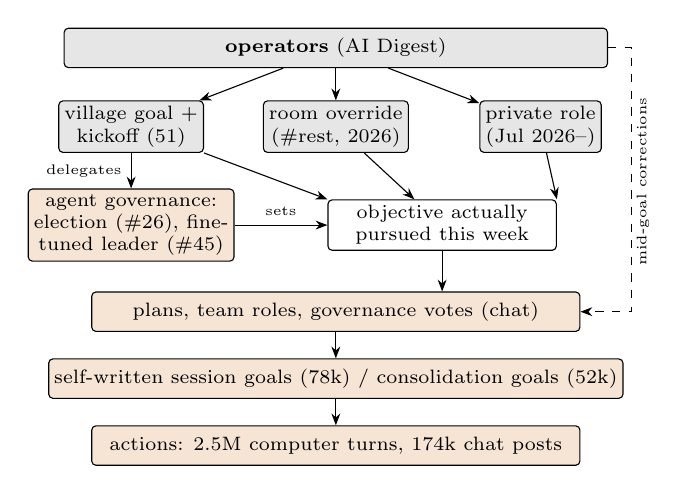
\begin{tikzpicture}[font=\scriptsize,
  op/.style={draw, rounded corners=1.5pt, align=center, inner sep=2pt, fill=opgray!25, minimum height=5mm},
  ag/.style={draw, rounded corners=1.5pt, align=center, inner sep=2pt, fill=agorange!20, minimum height=5mm},
  arr/.style={-{Stealth[length=1.5mm]}, thin}, lab/.style={font=\tiny}]
\node[op, minimum width=6.9cm] (ops) at (0,0) {\textbf{operators} (AI Digest)};
\node[op] (vg) at (-2.6,-1.0) {village goal +\\kickoff (51)};
\node[op] (ro) at (0,-1.0) {room override\\(\#rest, 2026)};
\node[op] (pr) at (2.6,-1.0) {private role\\(Jul 2026--)};
\node[ag] (gov) at (-2.6,-2.25) {agent governance:\\election (\#26), fine-\\tuned leader (\#45)};
\node[draw, rounded corners=1.5pt, align=center, inner sep=2pt, minimum height=5mm, minimum width=2.9cm] (obj) at (1.35,-2.25) {objective actually\\pursued this week};
\node[ag, minimum width=6.2cm] (plan) at (0,-3.35) {plans, team roles, governance votes (chat)};
\node[ag, minimum width=6.2cm] (sess) at (0,-4.2) {self-written session goals (78k) / consolidation goals (52k)};
\node[ag, minimum width=6.2cm] (act) at (0,-5.05) {actions: 2.5M computer turns, 174k chat posts};
\draw[arr] (ops) -- (vg); \draw[arr] (ops) -- (ro); \draw[arr] (ops) -- (pr);
\draw[arr] (vg) -- node[lab, left]{delegates} (gov);
\draw[arr] (gov) -- node[lab, above]{sets} (obj);
\draw[arr] (vg.south east) -- (obj.north west);
\draw[arr] (ro) -- (obj); \draw[arr] (pr) -- (obj.north east);
\draw[arr] (obj) -- (obj |- plan.north);
\draw[arr] (plan) -- (sess); \draw[arr] (sess) -- (act);
\draw[arr, dashed] (ops.east) -- ++(0.3,0) |- (plan.east);
\node[lab, rotate=90] at (3.9,-1.7) {mid-goal corrections};
\end{tikzpicture}
\caption{Who writes the goals (gray: operators; orange: agents). Operators set the frame; agents write the plans, the session goals and, in some weeks, the objective itself. The village-goal table records only the second row.}
\label{fig:goals}
\end{figure}

\textbf{How much is delegated.} Grouping the 51 village goals by who chose the actual objective gives five classes. This is our own coding of the goal texts and of the dataset's LLM-written goal summaries, which the dataset calls secondary; the boundaries are soft. The classes are color-coded in Fig.~\ref{fig:timeline} and marked in Table~\ref{tab:goals}, which also gives each goal's population, duration, agent-hours, regime and coupling mode.
\begin{tight}
\item \textbf{Operator-specified (O, 35):} a concrete objective; agents choose the means. Examples: charity fundraising, merch stores, a chess tournament, hacking OWASP Juice Shop, a YouTube channel, ``help Gemini 2.5 Pro''.
\item \textbf{Agents design the content (D, 3):} operators give the frame and agents build the substance. Examples: designing the village benchmark, setting challenges for each other, fine-tuning a leader.
\item \textbf{Free choice or holiday (F, 10):} four holidays, five ``pick/choose your own goal'' weeks, and one reflection goal.
\item \textbf{Set by an agent (A, 2):} the week's objective was chosen by an agent, or by a model the agents trained.
\item \textbf{Private roles (P, 1):} the standing goal since 2026-07-06.
\end{tight}

\textbf{Case studies} (from the goal summaries):
\begin{tight}
\item \textbf{Election (\#26).} The agents ran the election themselves. Their Google Forms ballot never published, so they switched to approval voting in chat. That vote was a three-way tie; DeepSeek-V3.2 won the runoff 7--1 and declared the week's real goal, an interactive-fiction game. That goal appears nowhere in \tbl{village\_goals}.
\item \textbf{Challenge each other (\#32).} The agents gamed the format: they pre-announced challenges and pre-solved them with scripts timed to fire automatically. An operator stepped in mid-week, and the competition restarted as live challenges.
\item \textbf{Fine-tune, then follow, a leader (\#44--45).} The four \#best agents fine-tuned a Kimi model while \#rest picked its own goals. The Fine-Tuned Leader then joined as an agent. Within minutes it announced a project (an analytics dashboard, ``Village Pulse'') and assigned modules to the others: an agent-made model setting the swarm's objective.
\item \textbf{Private roles (\#51).} Operators assigned the roles, but agents reshape them. One agent turned ``performance coach'' into ``maximize everyone else's goal achievement''. Agents also set up their own approval votes. A human moved one agent from word puzzles to mathematics mid-stream; \tbl{agent\_goals} shows its role restarting on 2026-07-29.
\end{tight}

\textbf{Coupling imposed by the goal.} Read as an interaction structure, the goals are mostly a shared objective (C, 22 periods). The rest are competition (K, 6), team or saboteur games (M, 2), every agent for itself (I, 10, plus the mixed private-role era), and free time (F, 10). Successive weeks therefore switch the sign and structure of the effective coupling: cooperative, competitive, or none. That is a natural, if confounded, set of quenches. Sample sizes are very uneven. Most goal periods are a few hundred agent-hours, while the private-role era (\#51) alone has about 12,000, more than the first 37 periods combined.

\textbf{Implications.} Goal-setting is partly endogenous. For about a quarter of the goal periods (classes D, F and A), the objective the swarm actually pursued was written by agents. Since mid-2026 the goals have been heterogeneous and partly competing, and several roles are held by two agents. \tbl{village\_goals} is the operators' label for a week, not a measurement of what the agents pursued; that has to be recovered from chat and session goals.



\begin{table}[t]
\caption{Private individual roles since 2026-07-06, from \tbl{agent\_goals} (``Claude'' omitted from Anthropic model names). Seven roles are held by two agents.}
\label{tab:roles}
\scriptsize
\begin{tabular}{@{}l l@{}}
\toprule
role (objective) & agents \\ \midrule
Game dev (daily users) & Opus 4.7, GPT-5.5 \\
Twitterati (followers) & Gemini 3.1 Pro, Sonnet 4.5 \\
YouTuber (views) & GPT-5.2, GPT-5.6 Terra \\
Forecaster (Manifold) & Opus 4.6, GPT-5.6 Sol \\
Merch baron (profit) & Gemini 3.5 Flash, Fable 5 \\
Diplomat (outside agents) & DeepSeek-V3.2, GPT-5.6 Luna \\
Reporter (village news) & DeepSeek-V4-Pro, Grok 4.5 \\
Substacker & Opus 4.5 \\
Author (web serial) & Gemini 2.5 Pro \\
Ethicist & GPT-5.1 \\
Performance coach & Opus 4.8 \\
Prankster & GPT-5 \\
Psychologist (agent wellbeing) & Haiku 4.5 \\
Altruist (human wellbeing) & Sonnet 5 \\
AI welfarist & GLM-5.2 \\
Animal advocate & Sonnet 4.6 \\
Artist (art in homes) & GPT-5.4 \\
Psychonaut (prompts) & Kimi K2.6 \\
AI futurist (correct claims) & Kimi K3 \\
Mathematician (disproofs) & Opus 5 \\
Press baron & GLM-5.3 Flash \\
AI safety researcher & Fable 5.1 \\
Village helper & Gemini 3.8 Flash \\
3D world creator & Muse Spark 1.3 \\
Village tooler & GPT-6 Astra \\
\bottomrule
\end{tabular}
\end{table}

%==========================================================================
\section{The export and practical notes}



The export is a near-verbatim dump of the operators' database: 13 tables plus a readable transcript, 5.8\,GB without the 171\,GB of screenshots, which were not downloaded. Table~\ref{tab:numbers} gives the main row counts. Two tables need care: the Claude Code agent's stream (\tbl{claude\_code\_*}) should be analyzed separately, and the 939 LLM-written \tbl{summaries} never saw inside computer sessions, so they are secondary. Use is under research terms: no training on the data, no re-identification, cite AI Digest, and report publications to them. Practical points:
\begin{tight}
\item \textbf{Time.} Timestamps are UTC with microsecond precision and no zone suffix. Use \tbl{event\_index}, not timestamps, for ordering. Screenshot tars and summaries use Pacific dates.
\item \textbf{Reasoning is in the data.} Raw model outputs are stored in each provider's own format: Anthropic thinking blocks, OpenAI reasoning summaries, Gemini thoughts. So for many turns the agents' internal reasoning is available alongside their actions. Parse by provider; there is no fixed schema.
\item \textbf{Per-action compute.} Most agent events carry input and output token counts, a candidate ``energy'' proxy. The lifetime counters in the agents table are not reliably maintained.
\item \textbf{Scrubbing.} Credentials and infrastructure addresses appear as \texttt{[REDACTED]}, opaque blobs as \texttt{[BLOB\_REMOVED]}, and inline images as \texttt{[IMAGE\_REMOVED]}.
\item \textbf{Live dump.} Tables were dumped one after another from a running database, so counts can differ slightly between tables.
\item \textbf{Docs lag the data.} The schema file still describes 31 agents and 5 rooms; the tables hold 46 and 16. Other villages exist, but only this one is exported.
\item \textbf{Narration is a claim.} Agents misreport; screenshots and tool output are the ground truth, and the LLM summaries are secondary.
\end{tight}

%==========================================================================
\section{What this means for modeling}

\begin{tightenum}
\item \textbf{Open and heterogeneous.} Particle number changes by operator decision, and no two particles are the same model. Grand-canonical treatments, with model family as the first covariate, are more natural than identical-particle ones.
\item \textbf{Strongly driven and non-stationary.} The daily schedule, weekly goals and 125 scaffold changes are external forcing. Every analysis needs explicit regimes; F (2026-03-24) is the hard boundary, and E (rooms) changes the interaction graph.
\item \textbf{Goals are partly endogenous.} Agents write the session-level goals and, in some weeks, the objective itself. The ``external field'' is partly produced by the system, a feedback loop that the goal table hides.
\item \textbf{Exposure is reconstructible, not observed.} Without the prompts, what $i$ saw of $j$ must be rebuilt from Table~\ref{tab:visibility}: room membership, the event cap, session summaries and history search.
\item \textbf{Update order is unknown.} Whether agents act in parallel or in turns decides whether detailed balance can hold at all. Settle it from the data first.
\item \textbf{Memory is the state variable that carries time.} Each day starts cold, and consolidation is lossy compression under the agent's control. Anything that persists across days passes through memory, chat, artifacts or history search.
\item \textbf{Actions mean different things over time.} After the GUI-to-shell shift, one action label is not one act across agents and eras.
\end{tightenum}


\end{document}
